\documentclass{standalone}

\usepackage[latin1]{inputenc}
\usepackage{tikz}

\usetikzlibrary{calc}

% GNUPLOT required
\begin{document}
\pagestyle{empty}

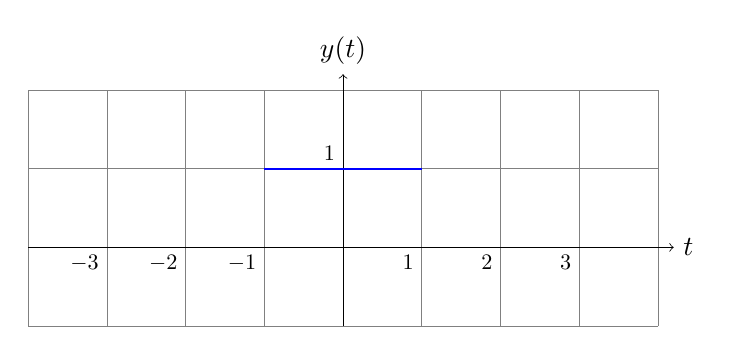
\begin{tikzpicture}[line width=0.25mm]
    \draw[very thin,color=gray] (-4,-1) grid (4,2);
    \draw[->, line width=0.1mm] (-4,0) -- (4.2,0) node[right] {$t$};
    \draw[->, line width=0.1mm] (0,-1) -- (0,2.2) node[above] {$y(t)$};

	% x(t)
    \draw[color=blue, domain=-3:-1] plot[id=x] function{0.5*x+1.5};
    \draw[color=blue, domain=1:3] plot[id=x] function{-0.5*x+1.5};
    
	\draw[color=blue] (-1,1) -- (1,1);
	
	%\draw[color=blue, domain=5:3.5] plot[id=x] function{0};% Para indicar la fucnción, se puede quitar los comentario y el último ;
        %node[above right] {$x(t)$};


	\foreach \x in {-3,...,-1,1,2,...,3} {%
    \draw ($(\x,0) + (0,0)$) -- ($(\x,0) + (0,0)$)
        node [below left,scale=0.8] {$\x$};
	}
	\foreach \y in {1} {%
    \draw ($(0,\y) + (0,0)$) -- ($(0,\y) + (0,0)$)
        node [above left,scale=0.8] {$\y$};
	}

\end{tikzpicture}


\end{document}
